%!TEX root =  ../main.tex
\renewcommand{\columnseprule}{1.5pt}
\begin{multicols*}{2}
\rule[0.4\baselineskip]{0.4\textwidth}{1pt}
\noindent
\LabSection{Log Infection}\label{sec:0704p}
\begin{exercises}{sec:0704p}
\lab{} Pathologists create designer virus to kill off certain bacteria and visa-versa.  The growth model of one pathogenic bacteria is shown by the function $P(t) = 2*3^{t/2}$, where $P$ is the population size in million, $t$ days after starting from a seed culture of 2 million.  Plot an accurate graph, using a $y$-scale of 1:1, and an $x$-scale of 1:3.

\noindent
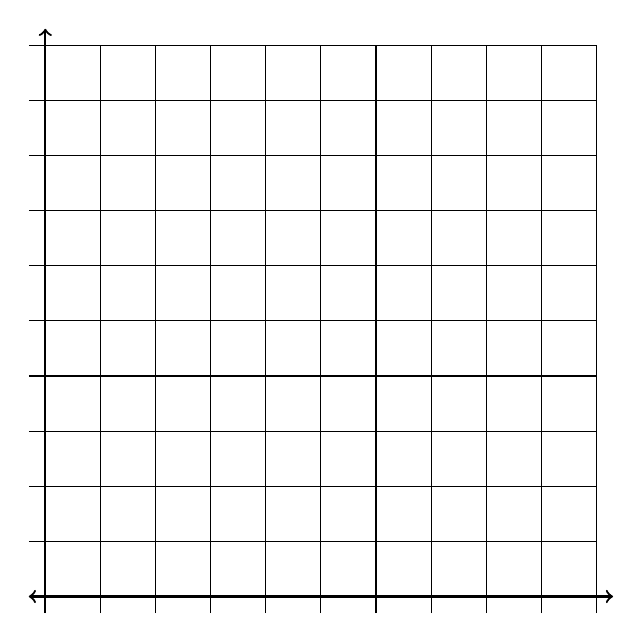
\begin{tikzpicture}[xscale=0.7,yscale=0.7]
	\draw [thick, <->] (-0.3,0) -- (10.3,0);
	\draw [thick, ->] (0,-0.3) -- (0,10.3);
	\draw [thin] (-0.3,-0.3) grid (10,10);
\end{tikzpicture}

\lab{} The cure for this lethal bacteria is a virus, which can be modeled by the function $Q(t) = 5*2^{3t-7}$.  (Part of this function shows that the scientist was late in starting this culture, and so started with much more virus in the seed culture.)  Plot $g(x)$ on the same graph above.

\vspace{2cm}
\lab{} Begin by setting the two equations equal to each other, in order to find their intersection.  What is the only option for algebraic manipulation when the variable is in the exponent?  (Multiplying or dividing both sides will yield no meaningful changes.)

\vspace{3cm}
\lab{} Using the properties of logarithms, expand both sides fully.  Also distribute the parentheses originating from the binomial exponent.  You should have 2 terms on the P side and 3 on the Q side.

\vspace{3cm}
\lab{} S.I.F.T. for $t$ and clear the complex fraction.

\vspace{5cm}
\lab{} Calculate a decimal answer and confirm graphically with the INTERSECT feature on your TI-8*.  Answer in Days/Hours/Minutes.

\vspace{3cm}
\lab{} Summarize what you learned in this problem set about exponential equation manipulation, using whole sentences.

\end{exercises}
\end{multicols*}